\documentclass[11pt]{article}
\usepackage{physics}
\usepackage[margin=1in]{geometry}
\usepackage[colorlinks= true, linkcolor = blue, urlcolor = blue]{hyperref}
\usepackage{graphicx}
\usepackage{titling}

\setlength{\droptitle}{-1in}
\posttitle{\par\end{center}}
\title{Simulating Disease Spread with Simple Elastic Collisions}
\author{Daniel Darvish}
\date{}
\begin{document}
\maketitle
\section{Introduction}
COVID-19 is presently without a doubt on everyone's mind. Recently, simulations have appeared which attempt to simulate disease spread and show the effects of various containment strategies. ``Flattening the curve'' of epidemiological spread has been the subject of many of these analyses. I was inspired by the \href{https://www.washingtonpost.com/graphics/2020/world/corona-simulator/}{simulations done by the Washington Post}, and wrote my own simulations with the goal of further varying parameters and analyzing how that affects epidemiological simulation data. I examine the effect of varying parameters on the epidemiological curve, including the fraction of people practicing ``social distancing'' and the case fatality rate.
\section{Simulation}
In these simulations, people are represented by moving or stationary disks which can elastically collide with each other, transmitting disease in the process. Fig.~\ref{fig:sim_ex_1} shows a picture of one such simulation in progress. When a red ``sick'' disk collide with a blue ``healthy'' disk, it transmit its disease with some probability $P_{t}$. When a person is infected, they will die with some probability $P_d$. After some amount of time $t_r$, a sick person will recover. In implementing a social distancing factor, some fraction $F_{q}$ are ``quarantined'' and therefore not permitted to move. The reader is encouraged to view a \href{https://www.youtube.com/watch?v=YYKz1-txdYw}{video of an example simulation}. The code for the simulation is available ~\href{https://github.com/dannydarvish/battelle_covid}{here}.

\begin{figure}[h]

    \centering
    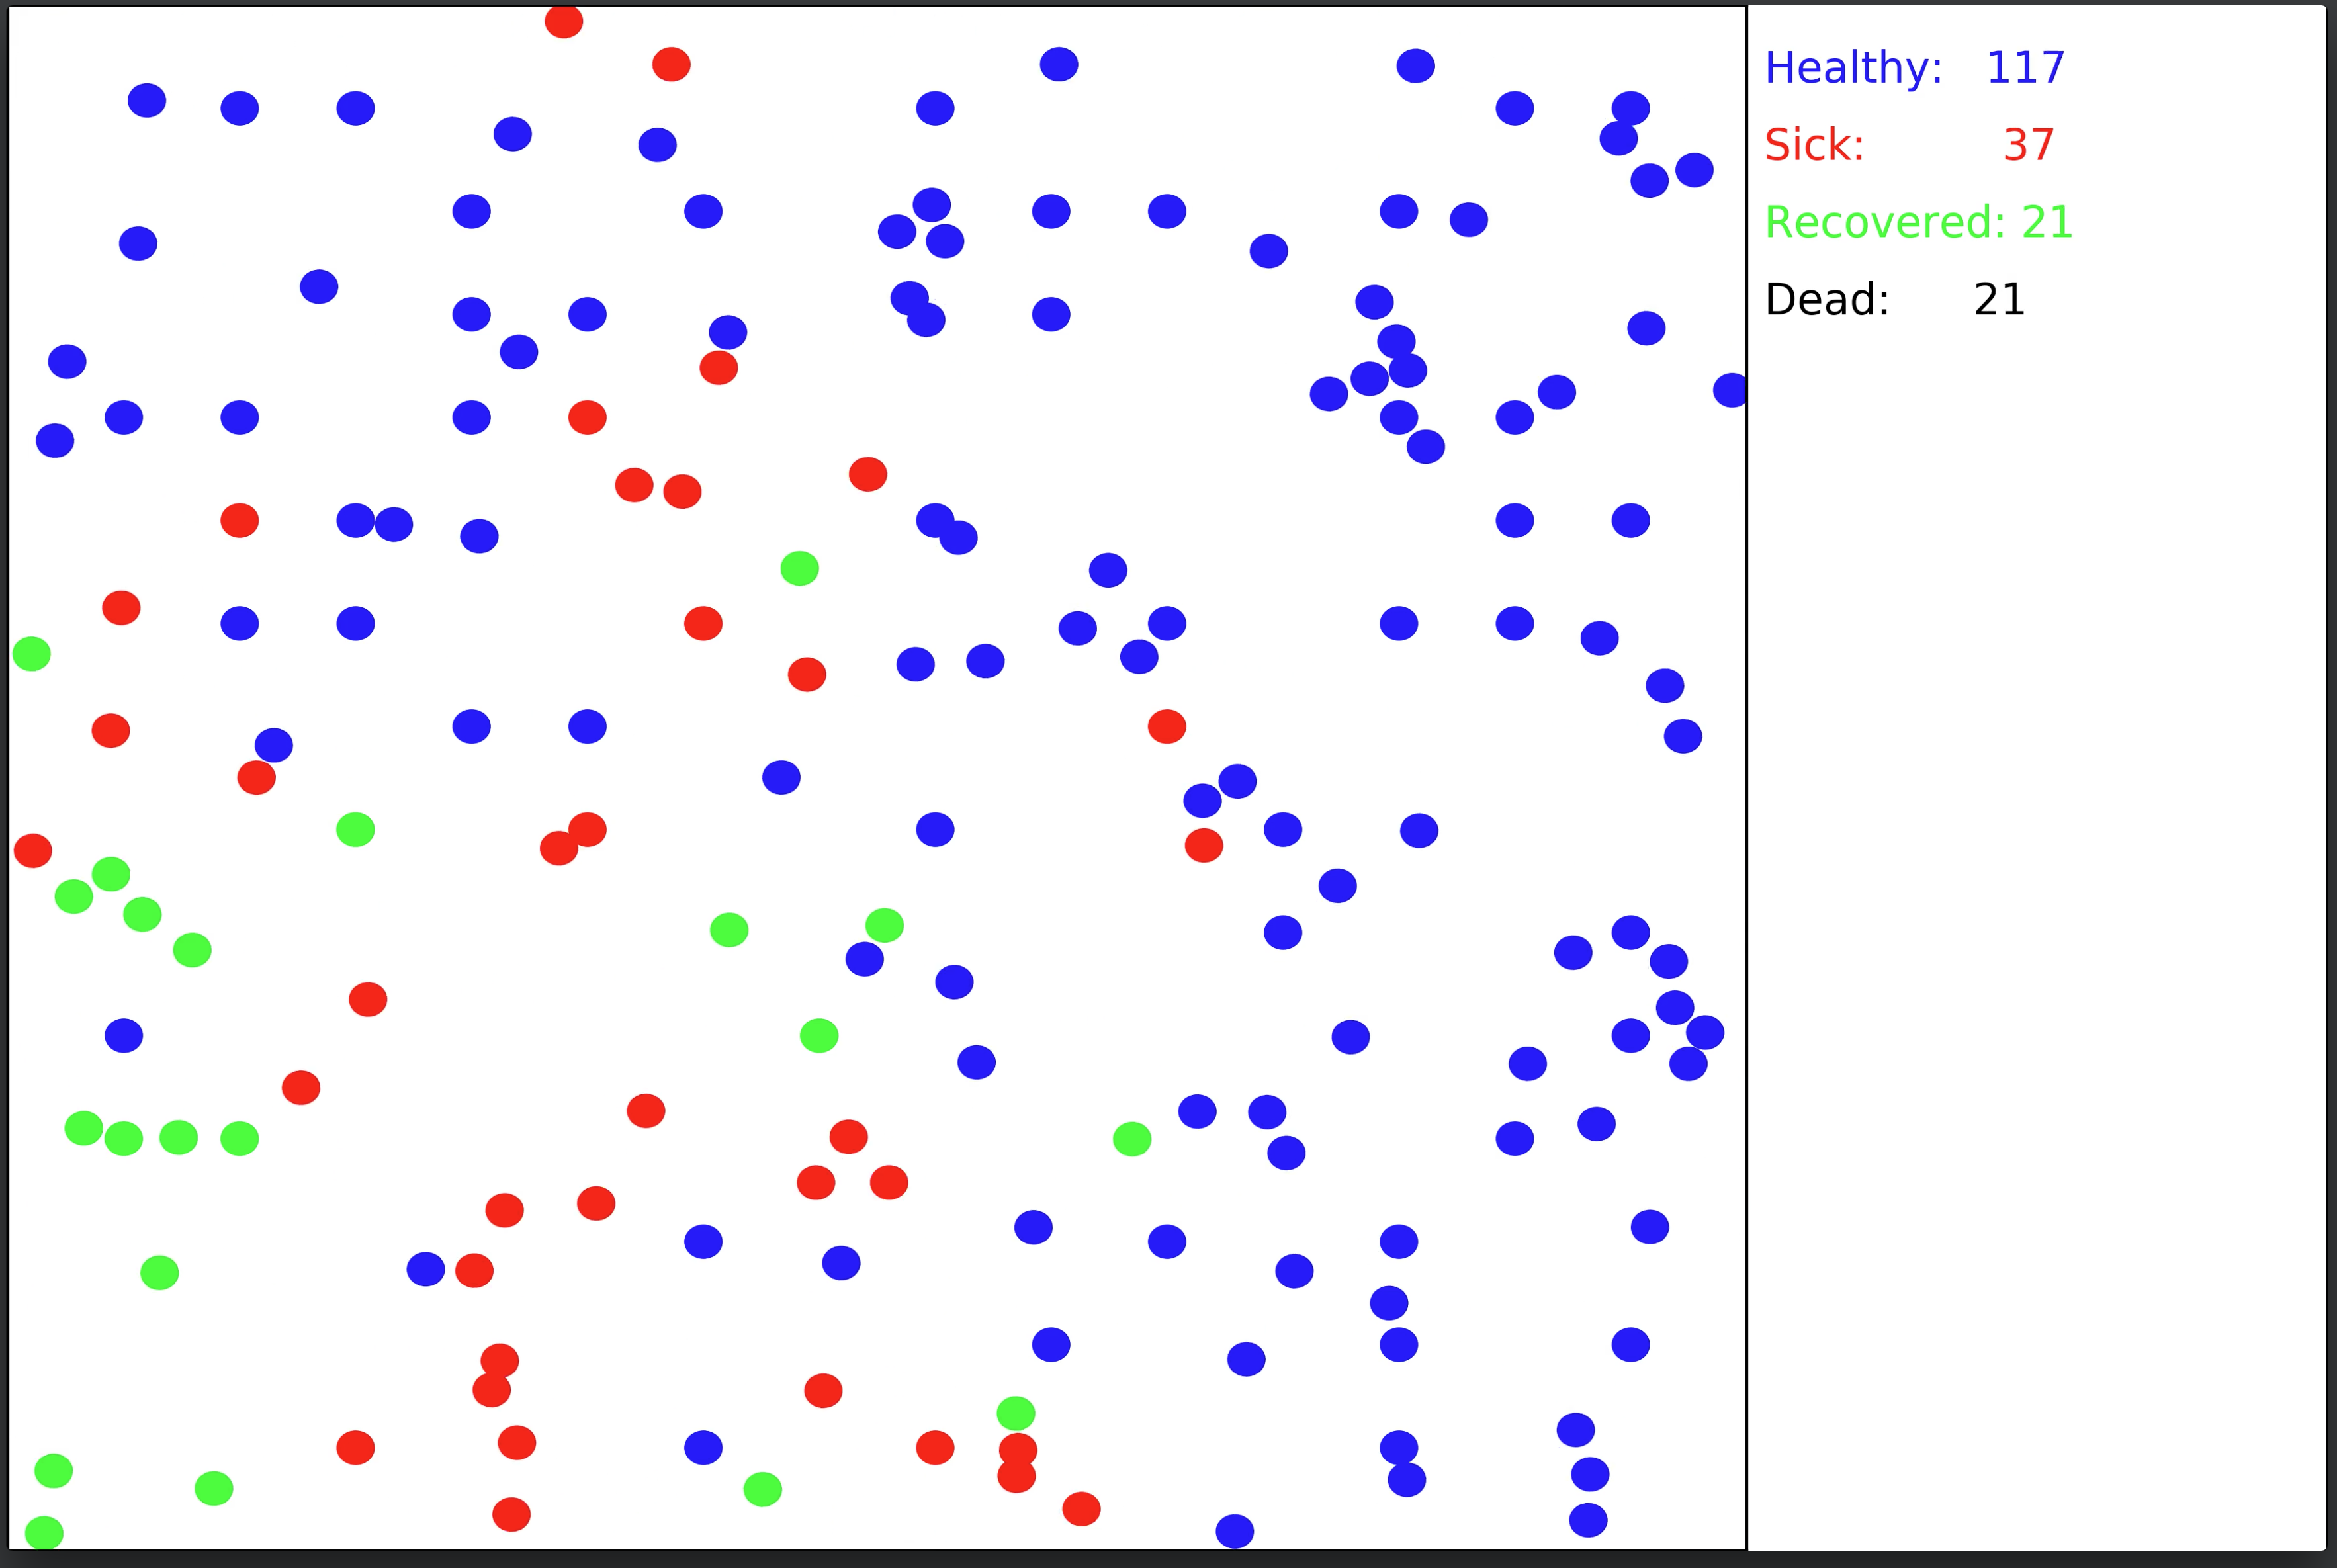
\includegraphics[scale=0.15]{figs/sim_ex_1.png}
    \caption{Example simulation in progress.}\label{fig:sim_ex_1}
\end{figure}
\section{Analysis}
\subsection{Flattening the curve via social distancing}
As an exercise, we wish to view how varying degrees of social distancing can reduce the peak of the curve of number sick vs. time. Flattening the curve in the real world is essential to ensuring we do not overwhelm our healthcare system. Fig.~\ref{fig:flatten} demonstrates the results of varying the fraction of those who practice social distancing, $F_q$, on the total curve of number sick vs. time. It is clear from the data that social distancing has a drastic effect on how acutely overwhelmed a population will be over the course of a pandemic.
\begin{figure}[h]
    \centering
    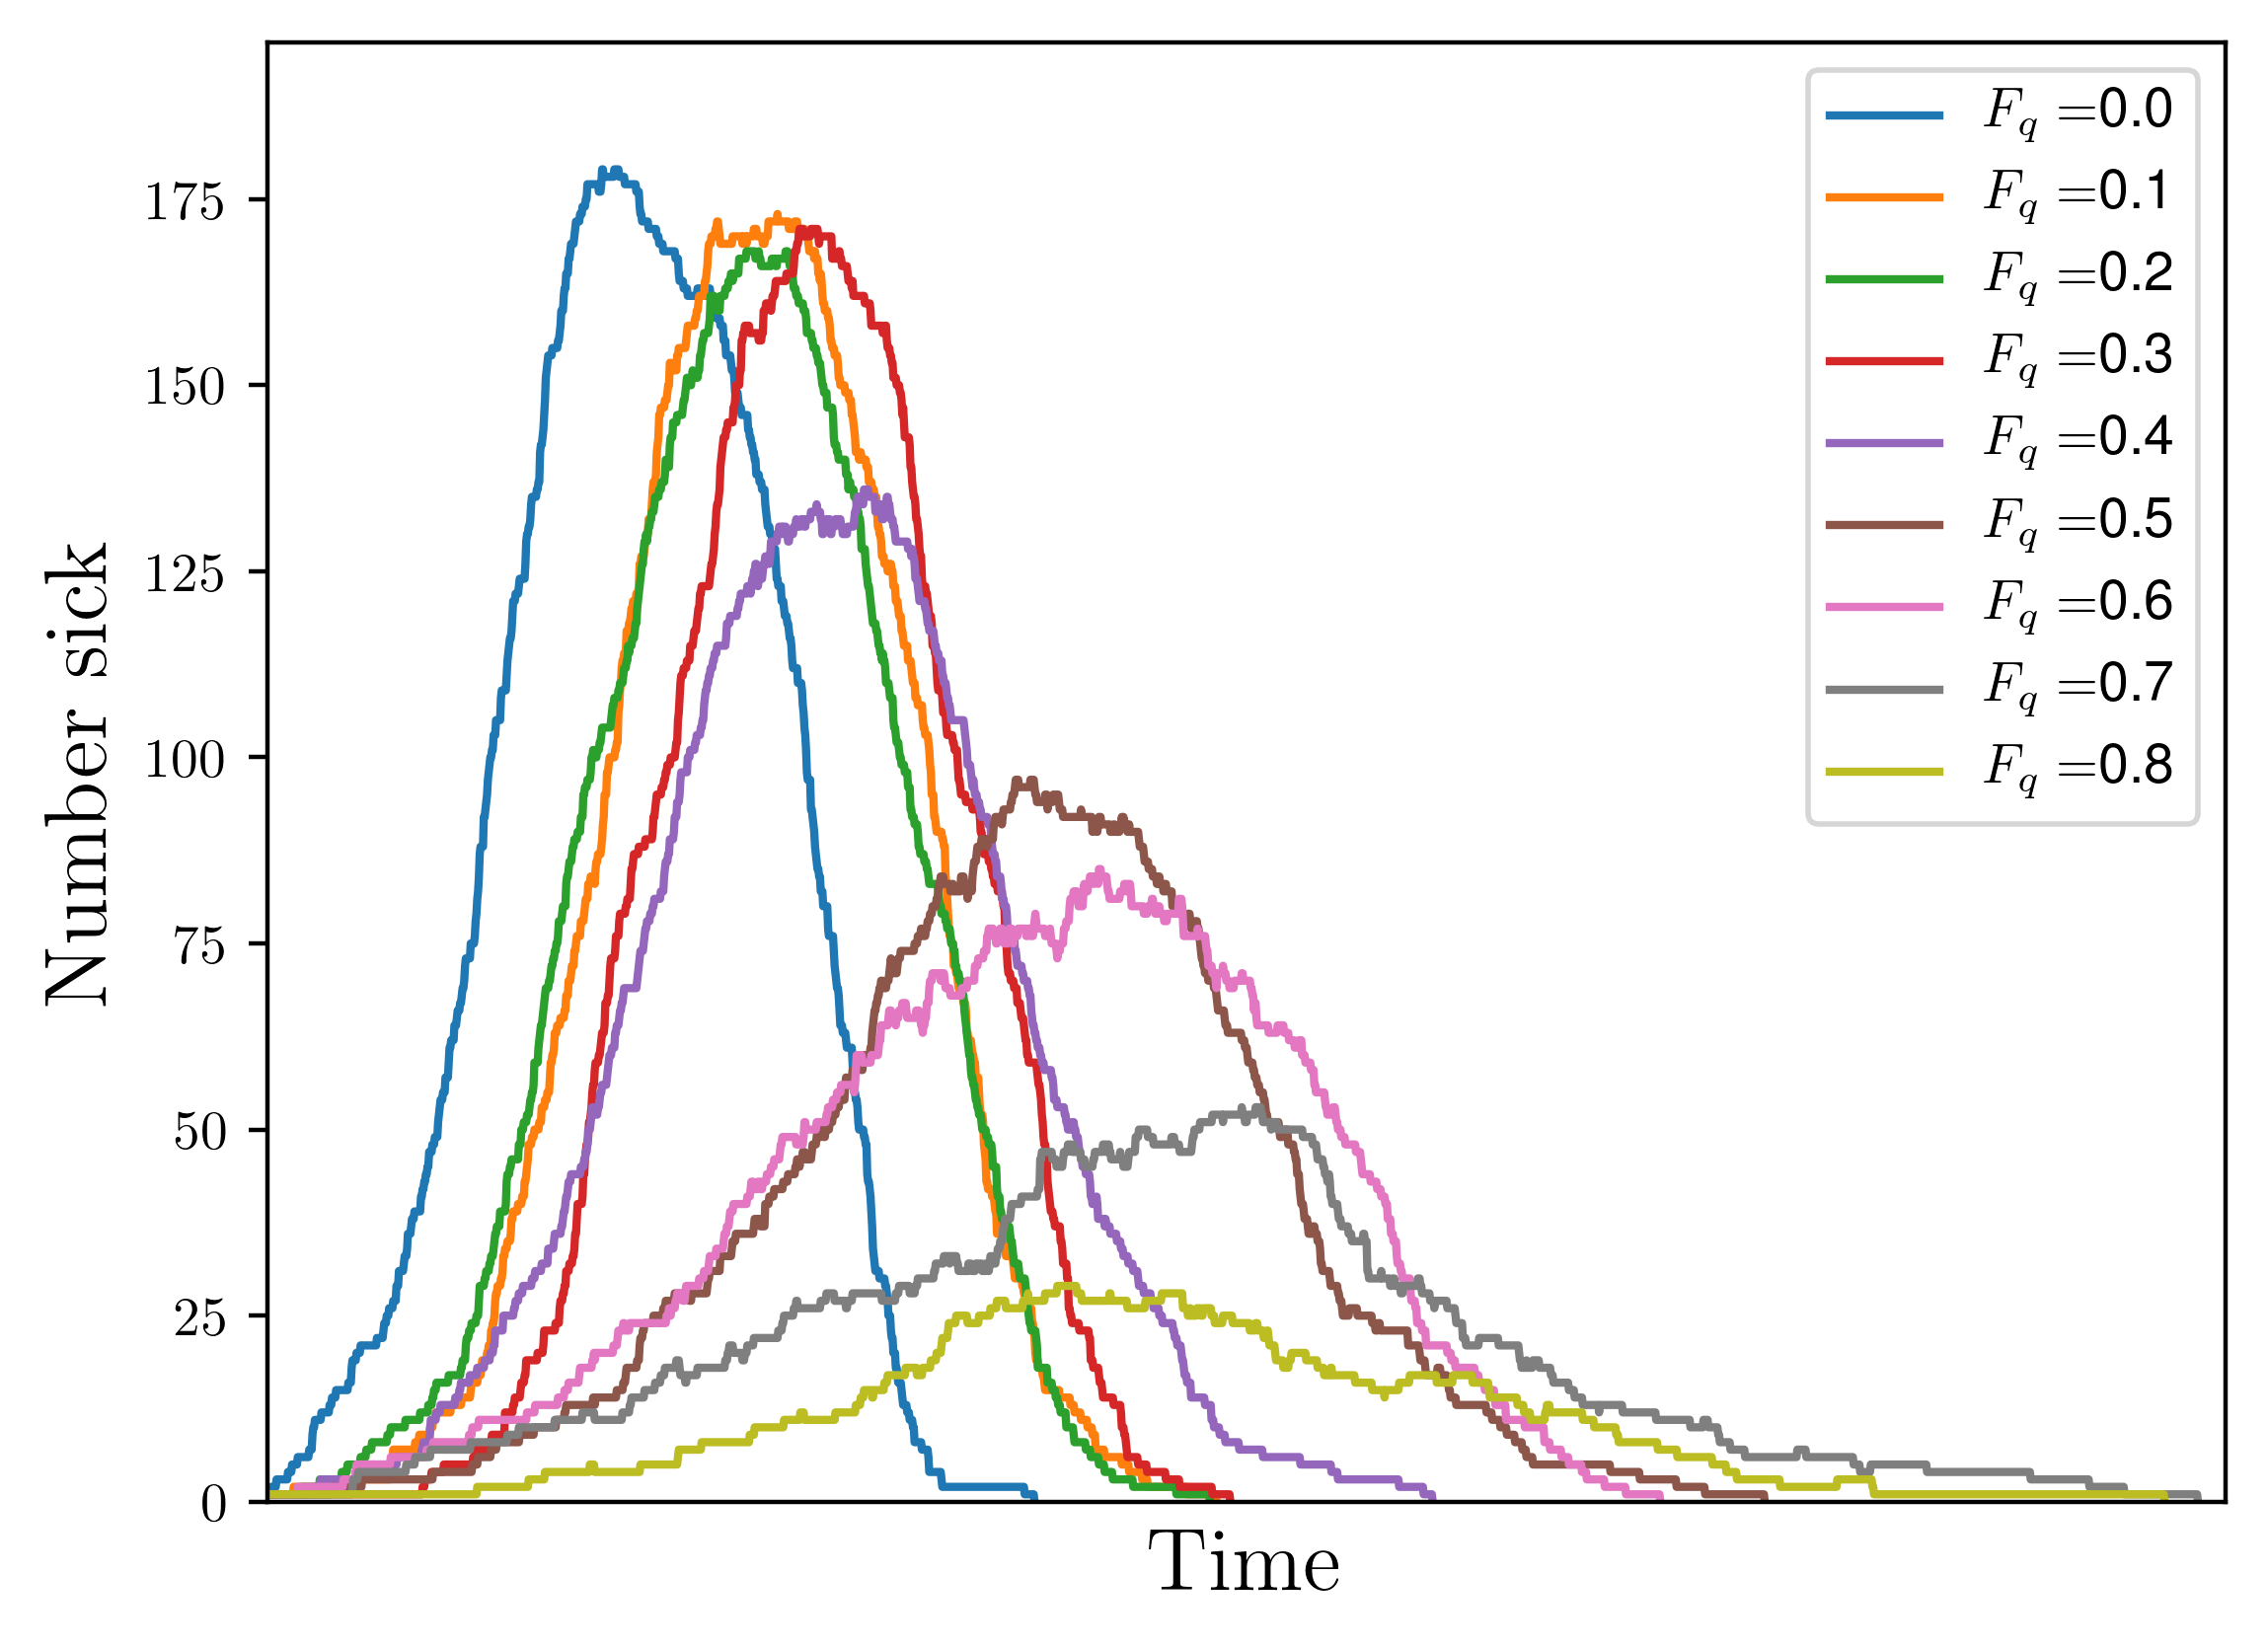
\includegraphics[scale=.6]{figs/flatten.png}
    \caption{The effect of social distancing on the epidemiological curve.}\label{fig:flatten}
\end{figure}
\subsection{Examining how less fatal diseases can be more deadly}
The virus that causes COVID-19 is genetically very similar to the virus that caused the deadly SARS epidemic. Interestingly, SARS has a much higher case fatality ratio than COVID-19, but COVID-19 has proven to be much more deadly on a global scale. To illustrate this paradox, we examine how varying the case fatality ratio of our simulation, $P_d$, affects the total number of fatalities. Fig.~\ref{fig:death_vs_cfr} illustrates what we might intuitively expect, that case fatality rate increases the total number of fatalities until a critical point at which people die too quickly to transmit disease.
\begin{figure}[h]
    \centering
    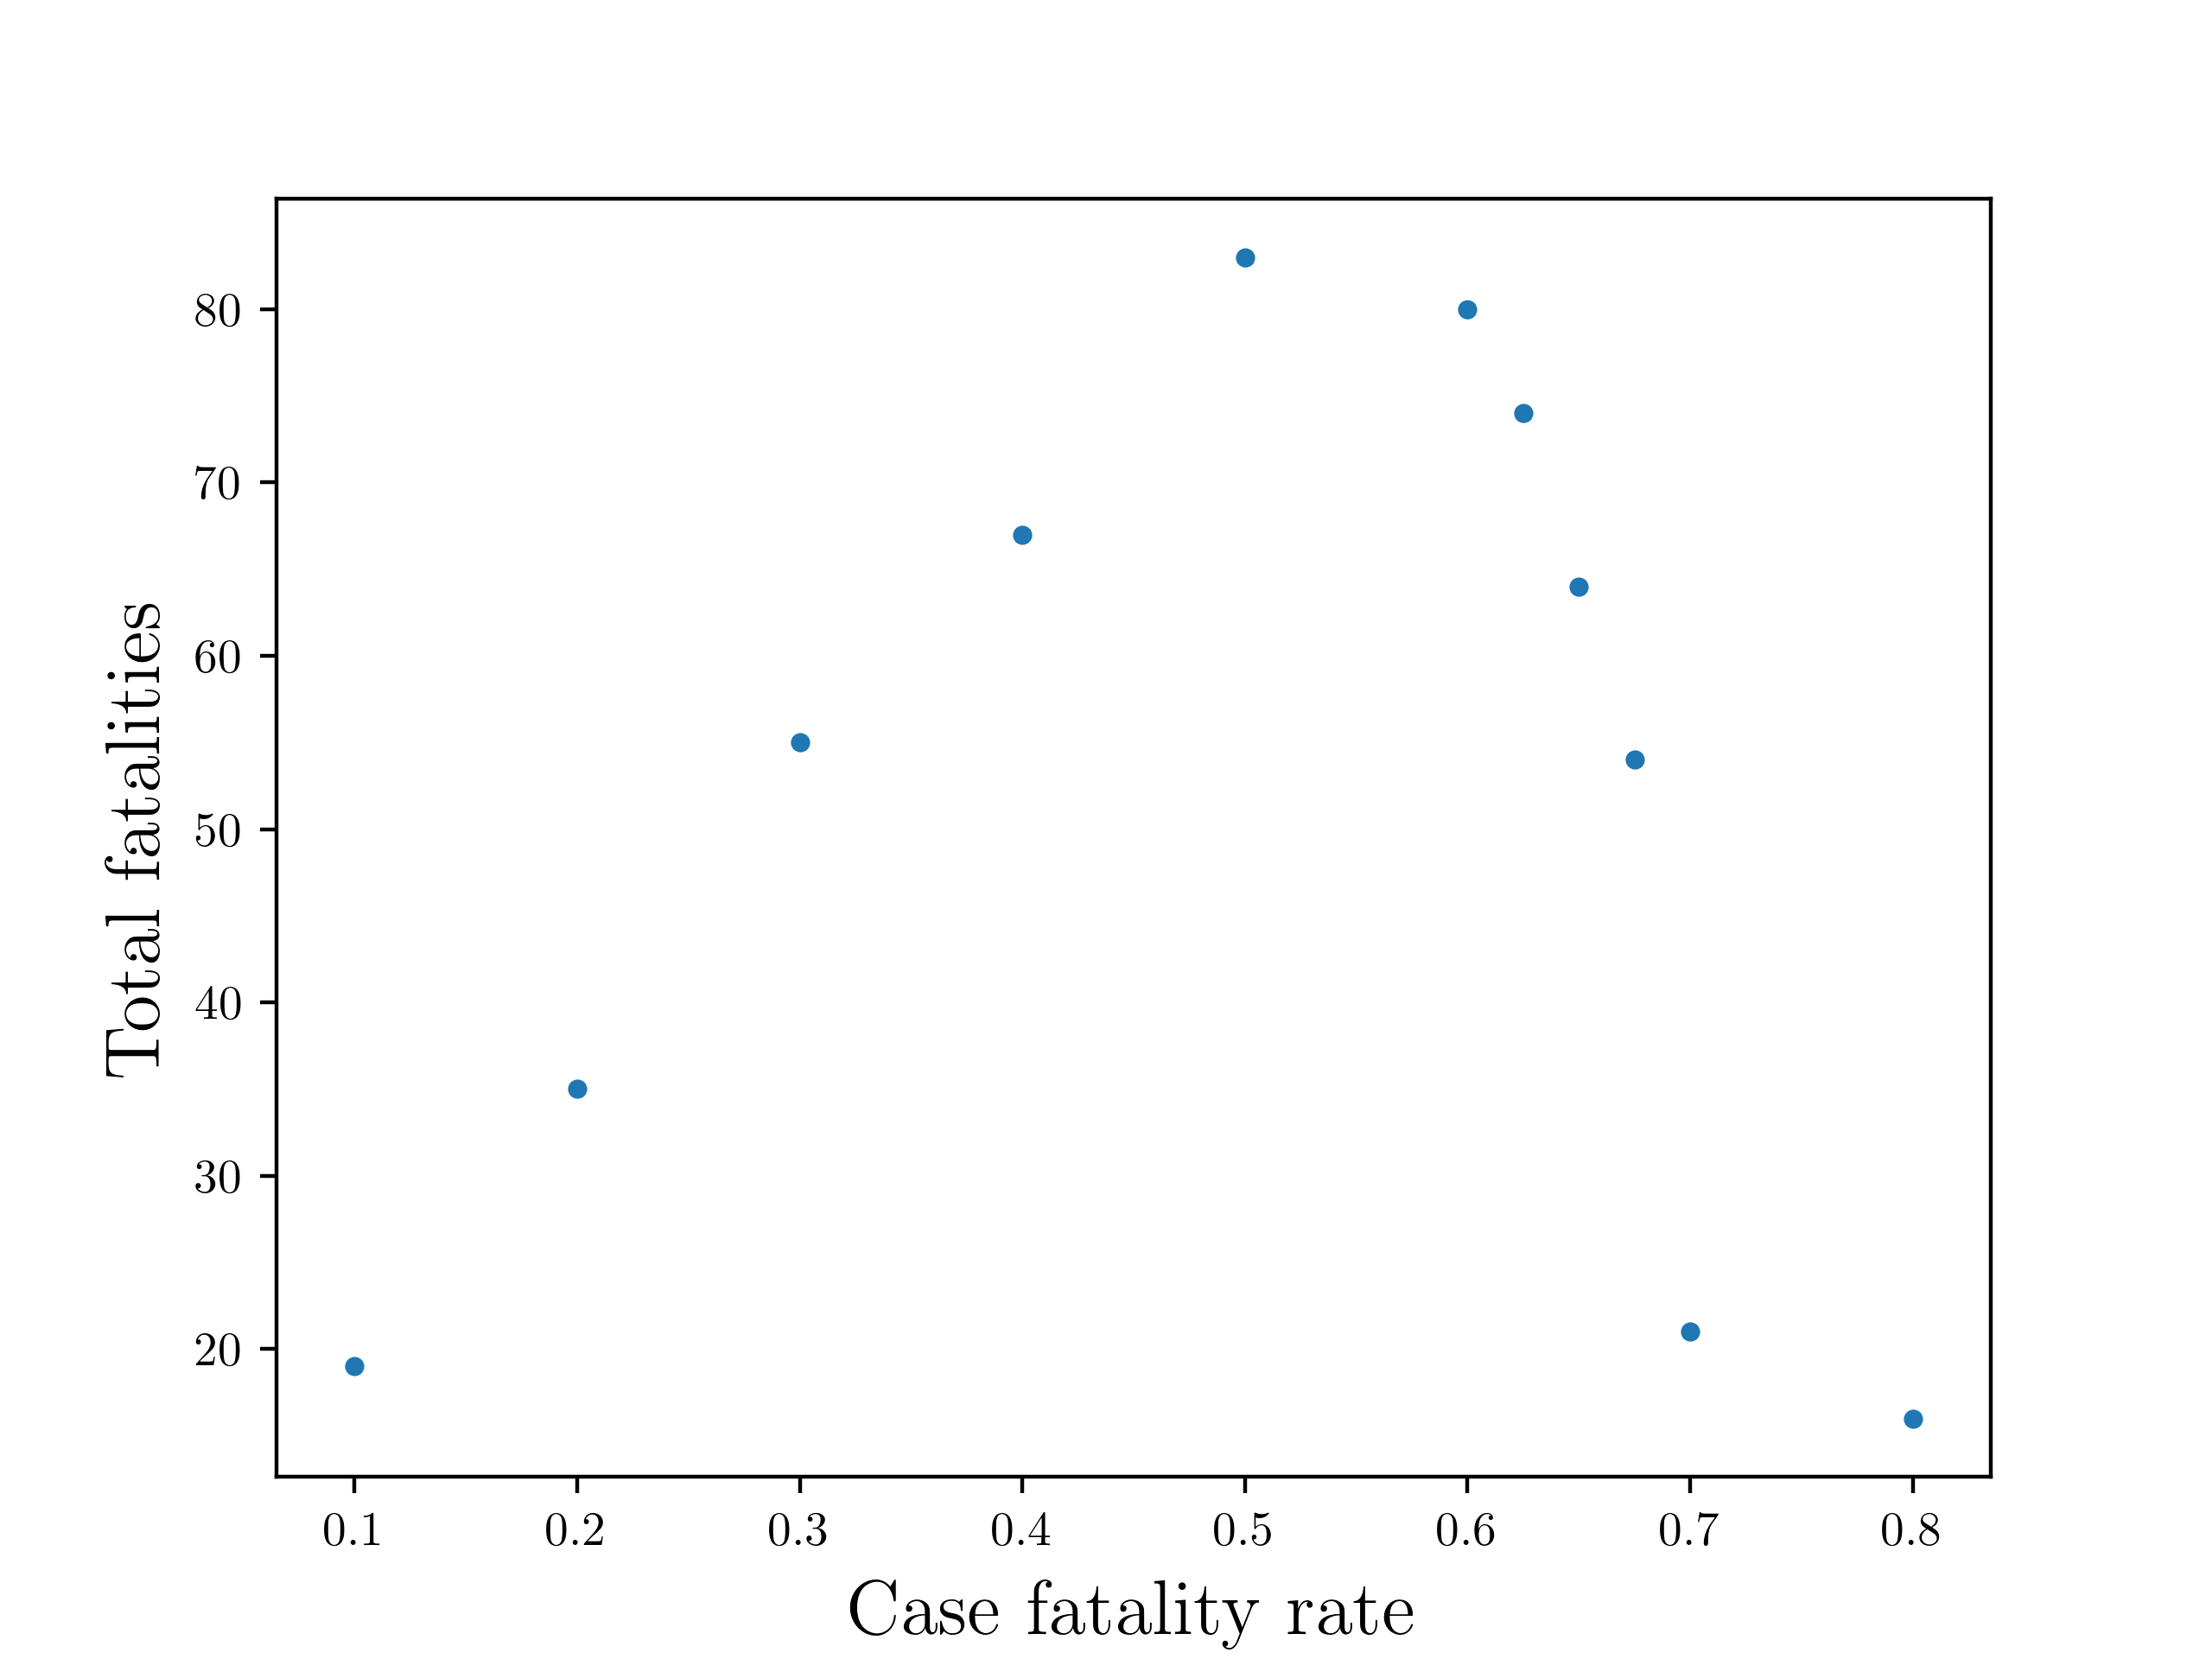
\includegraphics[scale=.6]{figs/total_deaths.png}
    \caption{Total number of fatalities vs. individual case fatality rate.}\label{fig:death_vs_cfr}
\end{figure}
\subsection{Further analysis and validation}
While I am without the time required to generate the data and perform the subsequent analysis, my next step would be to validate the trends shown in Figs.~\ref{fig:flatten} and \ref{fig:death_vs_cfr}. For the former, I calculate the correlation coefficient of $F_q$ and the height of the peak in Fig.~\ref{fig:flatten}. I would then run an ensemble of several simulations for each set of parameters. (They would still differ due to the stochasticity of the initial physical conditions, e.g. velocity and perhaps position.) I would then compute a bootstrap variance of the correlation coefficient to rigorously validate the effect of social distancing and evaluate statistical significance. For the trend shown in Fig.~\ref{fig:death_vs_cfr}, I would first partition the data from the ensemble of simulations into several subsets, and confirm that the trend observed is consistent across the subsets.
\end{document} 